\batchmode
%
\providecommand{\VMD}{}%
\providecommand{\MDENGINE}{VMD} 

%
\providecommand{\cvnamdugonly}[1]{}%
\providecommand{\cvvmdugonly}[1]{}%
\providecommand{\cvrefmanonly}[1]{#1} 

%
\providecommand{\cvnamdonly}[1]{}%
\providecommand{\cvvmdonly}[1]{#1}%
\providecommand{\cvlammpsonly}[1]{} 

%
\providecommand{\cvscriptonly}[1]{#1} 

%
\providecommand{\cvnamebasedonly}[1]{#1} 


\documentclass[11pt]{article}
\RequirePackage{ifthen}


\usepackage[margin=1in]{geometry}


\usepackage[english]{babel}


\usepackage{amsmath}
\usepackage{amssymb}
\usepackage{mathrsfs}


\usepackage{times}
\usepackage{inconsolata}
\usepackage{mathptmx}


\usepackage{graphicx}
\usepackage{color}
\definecolor{background-color}{gray}{0.84}


\usepackage{comment}


\usepackage{makeidx}
\makeindex


\usepackage[stable]{footmisc}


\usepackage[pagebackref,colorlinks,citecolor=blue,hyperfootnotes=false]{hyperref}


\usepackage{array}
\usepackage{multirow}
\usepackage{booktabs}


\setcounter{secnumdepth}{3}
\setcounter{tocdepth}{5}





\pagecolor[gray]{.7}

\usepackage[latin1]{inputenc}



\makeatletter

\makeatletter
\count@=\the\catcode`\_ \catcode`\_=8 
\newenvironment{tex2html_wrap}{}{}%
\catcode`\<=12\catcode`\_=\count@
\newcommand{\providedcommand}[1]{\expandafter\providecommand\csname #1\endcsname}%
\newcommand{\renewedcommand}[1]{\expandafter\providecommand\csname #1\endcsname{}%
  \expandafter\renewcommand\csname #1\endcsname}%
\newcommand{\newedenvironment}[1]{\newenvironment{#1}{}{}\renewenvironment{#1}}%
\let\newedcommand\renewedcommand
\let\renewedenvironment\newedenvironment
\makeatother
\let\mathon=$
\let\mathoff=$
\ifx\AtBeginDocument\undefined \newcommand{\AtBeginDocument}[1]{}\fi
\newbox\sizebox
\setlength{\hoffset}{0pt}\setlength{\voffset}{0pt}
\addtolength{\textheight}{\footskip}\setlength{\footskip}{0pt}
\addtolength{\textheight}{\topmargin}\setlength{\topmargin}{0pt}
\addtolength{\textheight}{\headheight}\setlength{\headheight}{0pt}
\addtolength{\textheight}{\headsep}\setlength{\headsep}{0pt}
\setlength{\textwidth}{349pt}
\newwrite\lthtmlwrite
\makeatletter
\let\realnormalsize=\normalsize
\global\topskip=2sp
\def\preveqno{}\let\real@float=\@float \let\realend@float=\end@float
\def\@float{\let\@savefreelist\@freelist\real@float}
\def\liih@math{\ifmmode$\else\bad@math\fi}
\def\end@float{\realend@float\global\let\@freelist\@savefreelist}
\let\real@dbflt=\@dbflt \let\end@dblfloat=\end@float
\let\@largefloatcheck=\relax
\let\if@boxedmulticols=\iftrue
\def\@dbflt{\let\@savefreelist\@freelist\real@dbflt}
\def\adjustnormalsize{\def\normalsize{\mathsurround=0pt \realnormalsize
 \parindent=0pt\abovedisplayskip=0pt\belowdisplayskip=0pt}%
 \def\phantompar{\csname par\endcsname}\normalsize}%
\def\lthtmltypeout#1{{\let\protect\string \immediate\write\lthtmlwrite{#1}}}%
\newcommand\lthtmlhboxmathA{\adjustnormalsize\setbox\sizebox=\hbox\bgroup\kern.05em }%
\newcommand\lthtmlhboxmathB{\adjustnormalsize\setbox\sizebox=\hbox to\hsize\bgroup\hfill }%
\newcommand\lthtmlvboxmathA{\adjustnormalsize\setbox\sizebox=\vbox\bgroup %
 \let\ifinner=\iffalse \let\)\liih@math }%
\newcommand\lthtmlboxmathZ{\@next\next\@currlist{}{\def\next{\voidb@x}}%
 \expandafter\box\next\egroup}%
\newcommand\lthtmlmathtype[1]{\gdef\lthtmlmathenv{#1}}%
\newcommand\lthtmllogmath{\dimen0\ht\sizebox \advance\dimen0\dp\sizebox
  \ifdim\dimen0>.95\vsize
   \lthtmltypeout{%
*** image for \lthtmlmathenv\space is too tall at \the\dimen0, reducing to .95 vsize ***}%
   \ht\sizebox.95\vsize \dp\sizebox\z@ \fi
  \lthtmltypeout{l2hSize %
:\lthtmlmathenv:\the\ht\sizebox::\the\dp\sizebox::\the\wd\sizebox.\preveqno}}%
\newcommand\lthtmlfigureA[1]{\let\@savefreelist\@freelist
       \lthtmlmathtype{#1}\lthtmlvboxmathA}%
\newcommand\lthtmlpictureA{\bgroup\catcode`\_=8 \lthtmlpictureB}%
\newcommand\lthtmlpictureB[1]{\lthtmlmathtype{#1}\egroup
       \let\@savefreelist\@freelist \lthtmlhboxmathB}%
\newcommand\lthtmlpictureZ[1]{\hfill\lthtmlfigureZ}%
\newcommand\lthtmlfigureZ{\lthtmlboxmathZ\lthtmllogmath\copy\sizebox
       \global\let\@freelist\@savefreelist}%
\newcommand\lthtmldisplayA{\bgroup\catcode`\_=8 \lthtmldisplayAi}%
\newcommand\lthtmldisplayAi[1]{\lthtmlmathtype{#1}\egroup\lthtmlvboxmathA}%
\newcommand\lthtmldisplayB[1]{\edef\preveqno{(\theequation)}%
  \lthtmldisplayA{#1}\let\@eqnnum\relax}%
\newcommand\lthtmldisplayZ{\lthtmlboxmathZ\lthtmllogmath\lthtmlsetmath}%
\newcommand\lthtmlinlinemathA{\bgroup\catcode`\_=8 \lthtmlinlinemathB}
\newcommand\lthtmlinlinemathB[1]{\lthtmlmathtype{#1}\egroup\lthtmlhboxmathA
  \vrule height1.5ex width0pt }%
\newcommand\lthtmlinlineA{\bgroup\catcode`\_=8 \lthtmlinlineB}%
\newcommand\lthtmlinlineB[1]{\lthtmlmathtype{#1}\egroup\lthtmlhboxmathA}%
\newcommand\lthtmlinlineZ{\egroup\expandafter\ifdim\dp\sizebox>0pt %
  \expandafter\centerinlinemath\fi\lthtmllogmath\lthtmlsetinline}
\newcommand\lthtmlinlinemathZ{\egroup\expandafter\ifdim\dp\sizebox>0pt %
  \expandafter\centerinlinemath\fi\lthtmllogmath\lthtmlsetmath}
\newcommand\lthtmlindisplaymathZ{\egroup %
  \centerinlinemath\lthtmllogmath\lthtmlsetmath}
\def\lthtmlsetinline{\hbox{\vrule width.1em \vtop{\vbox{%
  \kern.1em\copy\sizebox}\ifdim\dp\sizebox>0pt\kern.1em\else\kern.3pt\fi
  \ifdim\hsize>\wd\sizebox \hrule depth1pt\fi}}}
\def\lthtmlsetmath{\hbox{\vrule width.1em\kern-.05em\vtop{\vbox{%
  \kern.1em\kern0.8 pt\hbox{\hglue.17em\copy\sizebox\hglue0.8 pt}}\kern.3pt%
  \ifdim\dp\sizebox>0pt\kern.1em\fi \kern0.8 pt%
  \ifdim\hsize>\wd\sizebox \hrule depth1pt\fi}}}
\def\centerinlinemath{%
  \dimen1=\ifdim\ht\sizebox<\dp\sizebox \dp\sizebox\else\ht\sizebox\fi
  \advance\dimen1by.5pt \vrule width0pt height\dimen1 depth\dimen1 
 \dp\sizebox=\dimen1\ht\sizebox=\dimen1\relax}

\def\lthtmlcheckvsize{\ifdim\ht\sizebox<\vsize 
  \ifdim\wd\sizebox<\hsize\expandafter\hfill\fi \expandafter\vfill
  \else\expandafter\vss\fi}%
\providecommand{\selectlanguage}[1]{}%
\makeatletter \tracingstats = 1 
\providecommand{\Tau}{\textrm{T}}
\providecommand{\Omicron}{\textrm{O}}
\providecommand{\Mu}{\textrm{M}}
\providecommand{\omicron}{\textrm{o}}
\providecommand{\Eta}{\textrm{H}}
\providecommand{\Chi}{\textrm{X}}
\providecommand{\Beta}{\textrm{B}}
\providecommand{\Epsilon}{\textrm{E}}
\providecommand{\Kappa}{\textrm{K}}
\providecommand{\Iota}{\textrm{J}}
\providecommand{\Zeta}{\textrm{Z}}
\providecommand{\Rho}{\textrm{R}}
\providecommand{\Nu}{\textrm{N}}
\providecommand{\Alpha}{\textrm{A}}


\begin{document}
\pagestyle{empty}\thispagestyle{empty}\lthtmltypeout{}%
\lthtmltypeout{latex2htmlLength hsize=\the\hsize}\lthtmltypeout{}%
\lthtmltypeout{latex2htmlLength vsize=\the\vsize}\lthtmltypeout{}%
\lthtmltypeout{latex2htmlLength hoffset=\the\hoffset}\lthtmltypeout{}%
\lthtmltypeout{latex2htmlLength voffset=\the\voffset}\lthtmltypeout{}%
\lthtmltypeout{latex2htmlLength topmargin=\the\topmargin}\lthtmltypeout{}%
\lthtmltypeout{latex2htmlLength topskip=\the\topskip}\lthtmltypeout{}%
\lthtmltypeout{latex2htmlLength headheight=\the\headheight}\lthtmltypeout{}%
\lthtmltypeout{latex2htmlLength headsep=\the\headsep}\lthtmltypeout{}%
\lthtmltypeout{latex2htmlLength parskip=\the\parskip}\lthtmltypeout{}%
\lthtmltypeout{latex2htmlLength oddsidemargin=\the\oddsidemargin}\lthtmltypeout{}%
\makeatletter
\if@twoside\lthtmltypeout{latex2htmlLength evensidemargin=\the\evensidemargin}%
\else\lthtmltypeout{latex2htmlLength evensidemargin=\the\oddsidemargin}\fi%
\lthtmltypeout{}%
\makeatother
\setcounter{page}{1}
\onecolumn

% !!! IMAGES START HERE !!!

{\newpage\clearpage
\lthtmlinlinemathA{tex2html_wrap_inline14027}%
$ \alpha $%
\lthtmlinlinemathZ
\lthtmlcheckvsize\clearpage}

\setcounter{secnumdepth}{3}
\setcounter{tocdepth}{5}
{\newpage\clearpage
\lthtmlinlinemathA{tex2html_wrap_inline14084}%
$ \,$%
\lthtmlinlinemathZ
\lthtmlcheckvsize\clearpage}


%
\providecommand{\key}[5]{%
  
  {\bf \large \tt #1 } $\langle\,$#3$\,\rangle$\  \\%
  {\bf Context: } #2 \\%
  {\bf Acceptable values: } #4 \\%
  {\bf Description: } #5}%


%
\providecommand{\keydef}[6]{%
  
  {\bf \large \tt #1 } $\langle\,$#3$\,\rangle$\  \\%
  {\bf Context: } #2 \\%
  {\bf Acceptable values: } #4 \\%
  {\bf Default value: } #5 \\%
  {\bf Description: } #6}%


%
\providecommand{\gradx}{\mbox{\boldmath$\nabla_{\!\!x}\,$}}%


%
\providecommand{\vx}{{\mbox{\boldmath{$x$}}}}%


%
\providecommand{\bm}[1]{{\mbox{\boldmath{$#1$}}}}%

\stepcounter{section}
\stepcounter{subsection}
\stepcounter{subsubsection}

%
\providecommand{\outputName}{\emph{outputName}}%


%
\providecommand{\restartName}{\emph{restartName}}%


%
\providecommand{\inputName}{\emph{inputName}}%

\stepcounter{section}
{\newpage\clearpage
\lthtmlinlinemathA{tex2html_wrap_inline14091}%
$ {\mbox{\boldmath {$x$}}}_{i}$%
\lthtmlinlinemathZ
\lthtmlcheckvsize\clearpage}

{\newpage\clearpage
\lthtmlinlinemathA{tex2html_wrap_inline14093}%
$ i$%
\lthtmlinlinemathZ
\lthtmlcheckvsize\clearpage}

{\newpage\clearpage
\lthtmlinlinemathA{tex2html_wrap_inline14095}%
$ 1$%
\lthtmlinlinemathZ
\lthtmlcheckvsize\clearpage}

{\newpage\clearpage
\lthtmlinlinemathA{tex2html_wrap_inline14097}%
$ N$%
\lthtmlinlinemathZ
\lthtmlcheckvsize\clearpage}

{\newpage\clearpage
\lthtmlinlinemathA{tex2html_wrap_indisplay14099}%
$\displaystyle \xi(t) \; = \xi\left({\mbox{\boldmath {$x$}}}_{i}(t), {\mbox{\boldmath {$x$}}}_{j}(t), {\mbox{\boldmath {$x$}}}_{k}(t),   \ldots \right)\;, \;\; 1 \leq i,j,k\ldots \leq N$%
\lthtmlindisplaymathZ
\lthtmlcheckvsize\clearpage}

{\newpage\clearpage
\lthtmlinlinemathA{tex2html_wrap_inline14103}%
$ d$%
\lthtmlinlinemathZ
\lthtmlcheckvsize\clearpage}

{\newpage\clearpage
\lthtmlinlinemathA{tex2html_wrap_inline14105}%
$ d_{1}$%
\lthtmlinlinemathZ
\lthtmlcheckvsize\clearpage}

{\newpage\clearpage
\lthtmlinlinemathA{tex2html_wrap_inline14107}%
$ d_{2}$%
\lthtmlinlinemathZ
\lthtmlcheckvsize\clearpage}

{\newpage\clearpage
\lthtmlinlinemathA{tex2html_wrap_inline14109}%
$ d = d_{1} - d_{2}$%
\lthtmlinlinemathZ
\lthtmlcheckvsize\clearpage}

{\newpage\clearpage
\lthtmlinlinemathA{tex2html_wrap_inline14111}%
$ C = +1$%
\lthtmlinlinemathZ
\lthtmlcheckvsize\clearpage}

{\newpage\clearpage
\lthtmlinlinemathA{tex2html_wrap_inline14113}%
$ C = -1$%
\lthtmlinlinemathZ
\lthtmlcheckvsize\clearpage}

{\newpage\clearpage
\lthtmlinlinemathA{tex2html_wrap_inline14115}%
$ c$%
\lthtmlinlinemathZ
\lthtmlcheckvsize\clearpage}

{\newpage\clearpage
\lthtmlinlinemathA{tex2html_wrap_inline14121}%
$ K$%
\lthtmlinlinemathZ
\lthtmlcheckvsize\clearpage}

{\newpage\clearpage
\lthtmlinlinemathA{tex2html_wrap_inline14127}%
$ w_d$%
\lthtmlinlinemathZ
\lthtmlcheckvsize\clearpage}

{\newpage\clearpage
\lthtmlinlinemathA{tex2html_wrap_inline14129}%
$ w_c$%
\lthtmlinlinemathZ
\lthtmlcheckvsize\clearpage}

{\newpage\clearpage
\lthtmlpictureA{tex2html_wrap14135}%
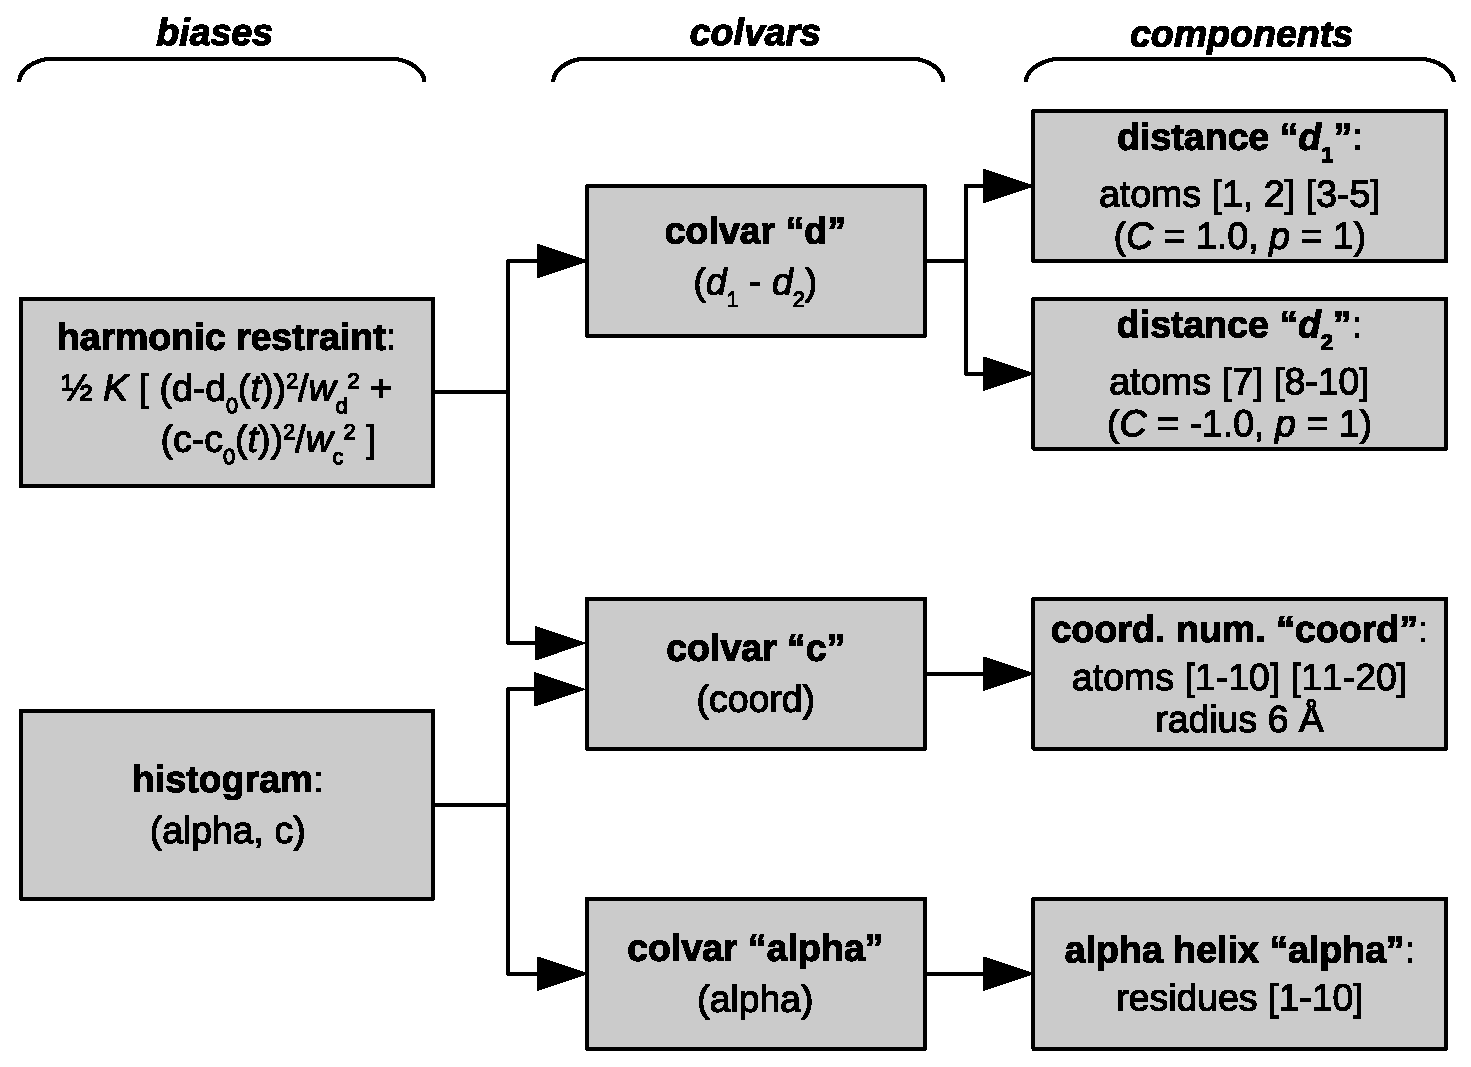
\includegraphics[width=12cm]{colvars_diagram}%
\lthtmlpictureZ
\lthtmlcheckvsize\clearpage}

\stepcounter{section}
\stepcounter{subsection}
{\newpage\clearpage
\lthtmlinlinemathA{tex2html_wrap_inline14139}%
$ <$%
\lthtmlinlinemathZ
\lthtmlcheckvsize\clearpage}

{\newpage\clearpage
\lthtmlinlinemathA{tex2html_wrap_inline14141}%
$ >$%
\lthtmlinlinemathZ
\lthtmlcheckvsize\clearpage}

\stepcounter{subsection}
{\newpage\clearpage
\lthtmlinlinemathA{tex2html_wrap_inline14232}%
$ \langle\,$%
\lthtmlinlinemathZ
\lthtmlcheckvsize\clearpage}

{\newpage\clearpage
\lthtmlinlinemathA{tex2html_wrap_inline14234}%
$ \,\rangle$%
\lthtmlinlinemathZ
\lthtmlcheckvsize\clearpage}

\stepcounter{subsection}
\stepcounter{subsection}
\stepcounter{section}
\stepcounter{subsection}
\stepcounter{subsection}
{\newpage\clearpage
\lthtmlinlinemathA{tex2html_wrap_inline14291}%
$ ^2$%
\lthtmlinlinemathZ
\lthtmlcheckvsize\clearpage}

\stepcounter{subsection}
\stepcounter{subsection}
{\newpage\clearpage
\lthtmlinlinemathA{tex2html_wrap_inline14363}%
$ k_B T / \sigma^2$%
\lthtmlinlinemathZ
\lthtmlcheckvsize\clearpage}

{\newpage\clearpage
\lthtmlinlinemathA{tex2html_wrap_inline14365}%
$ \sigma$%
\lthtmlinlinemathZ
\lthtmlcheckvsize\clearpage}

{\newpage\clearpage
\lthtmlinlinemathA{tex2html_wrap_inline14371}%
$ k_B T (\tau/2 \pi \sigma)^2$%
\lthtmlinlinemathZ
\lthtmlcheckvsize\clearpage}

{\newpage\clearpage
\lthtmlinlinemathA{tex2html_wrap_inline14373}%
$ \tau$%
\lthtmlinlinemathZ
\lthtmlcheckvsize\clearpage}

{\newpage\clearpage
\lthtmlinlinemathA{tex2html_wrap_inline14383}%
$ ^{-1}$%
\lthtmlinlinemathZ
\lthtmlcheckvsize\clearpage}

\stepcounter{subsection}
{\newpage\clearpage
\lthtmlinlinemathA{tex2html_wrap_inline14396}%
$ \xi_{i}$%
\lthtmlinlinemathZ
\lthtmlcheckvsize\clearpage}

{\newpage\clearpage
\lthtmlinlinemathA{tex2html_wrap_inline14398}%
$ \xi_{j}$%
\lthtmlinlinemathZ
\lthtmlcheckvsize\clearpage}

{\newpage\clearpage
\lthtmlinlinemathA{tex2html_wrap_inline14406}%
$ C_{i,j}(t)$%
\lthtmlinlinemathZ
\lthtmlcheckvsize\clearpage}

{\newpage\clearpage
\lthtmlinlinemathA{tex2html_wrap_inline14408}%
$ \left\langle \Pi\left(\xi_{i}(t_{0}),
        \xi_{j}(t_{0}+t)\right) \right\rangle$%
\lthtmlinlinemathZ
\lthtmlcheckvsize\clearpage}

{\newpage\clearpage
\lthtmlinlinemathA{tex2html_wrap_inline14414}%
$ \Pi(\xi_{i}, \xi_{j})$%
\lthtmlinlinemathZ
\lthtmlcheckvsize\clearpage}

{\newpage\clearpage
\lthtmlinlinemathA{tex2html_wrap_inline14416}%
$ (3\cos(\theta)^{2}-1)/2$%
\lthtmlinlinemathZ
\lthtmlcheckvsize\clearpage}

{\newpage\clearpage
\lthtmlinlinemathA{tex2html_wrap_inline14422}%
$ t$%
\lthtmlinlinemathZ
\lthtmlcheckvsize\clearpage}

{\newpage\clearpage
\lthtmlinlinemathA{tex2html_wrap_inline14424}%
$ \left\langle
      O\left(\xi_{i}, \xi_{j}\right) \right\rangle$%
\lthtmlinlinemathZ
\lthtmlcheckvsize\clearpage}

\stepcounter{section}
\stepcounter{subsection}
\stepcounter{subsection}
{\newpage\clearpage
\lthtmlinlinemathA{tex2html_wrap_inline14529}%
$ \mathbf{x}_{i}$%
\lthtmlinlinemathZ
\lthtmlcheckvsize\clearpage}

{\newpage\clearpage
\lthtmlinlinemathA{tex2html_wrap_inline14531}%
$ \xi$%
\lthtmlinlinemathZ
\lthtmlcheckvsize\clearpage}

{\newpage\clearpage
\lthtmlinlinemathA{tex2html_wrap_inline14533}%
$ \mathbf{x}_{i}' = R(\mathbf{x}_{i} - \mathbf{x}^{\mathrm{C}}) + \mathbf{x}^{\mathrm{ref}}$%
\lthtmlinlinemathZ
\lthtmlcheckvsize\clearpage}

{\newpage\clearpage
\lthtmlinlinemathA{tex2html_wrap_inline14535}%
$ \mathbf{x}^{\mathrm{C}}$%
\lthtmlinlinemathZ
\lthtmlcheckvsize\clearpage}

{\newpage\clearpage
\lthtmlinlinemathA{tex2html_wrap_inline14539}%
$ R$%
\lthtmlinlinemathZ
\lthtmlcheckvsize\clearpage}

{\newpage\clearpage
\lthtmlinlinemathA{tex2html_wrap_inline14541}%
$ \mathbf{x}^{\mathrm{ref}}$%
\lthtmlinlinemathZ
\lthtmlcheckvsize\clearpage}

{\newpage\clearpage
\lthtmlinlinemathA{tex2html_wrap_inline14571}%
$ _{\alpha}$%
\lthtmlinlinemathZ
\lthtmlcheckvsize\clearpage}

{\newpage\clearpage
\lthtmlinlinemathA{tex2html_wrap_inline14579}%
$ \partial{}R/\partial\mathbf{x}_{i}$%
\lthtmlinlinemathZ
\lthtmlcheckvsize\clearpage}

{\newpage\clearpage
\lthtmlinlinemathA{tex2html_wrap_inline14581}%
$ \partial\mathbf{x}^{\mathrm{C}}/\partial\mathbf{x}_{i}$%
\lthtmlinlinemathZ
\lthtmlcheckvsize\clearpage}

\stepcounter{subsection}
{\newpage\clearpage
\lthtmlinlinemathA{tex2html_wrap_inline14591}%
$ x$%
\lthtmlinlinemathZ
\lthtmlcheckvsize\clearpage}

{\newpage\clearpage
\lthtmlinlinemathA{tex2html_wrap_inline14593}%
$ y$%
\lthtmlinlinemathZ
\lthtmlcheckvsize\clearpage}

\stepcounter{subsection}
\stepcounter{section}
\stepcounter{subsection}
\stepcounter{subsubsection}
\stepcounter{subsubsection}
{\newpage\clearpage
\lthtmlinlinemathA{tex2html_wrap_inline14626}%
$ {\mbox{\boldmath {$r$}}}$%
\lthtmlinlinemathZ
\lthtmlcheckvsize\clearpage}

{\newpage\clearpage
\lthtmlinlinemathA{tex2html_wrap_inline14632}%
$ {\mbox{\boldmath {$r$}}}_1$%
\lthtmlinlinemathZ
\lthtmlcheckvsize\clearpage}

{\newpage\clearpage
\lthtmlinlinemathA{tex2html_wrap_inline14638}%
$ {\mbox{\boldmath {$r$}}}_2$%
\lthtmlinlinemathZ
\lthtmlcheckvsize\clearpage}

{\newpage\clearpage
\lthtmlinlinemathA{tex2html_wrap_inline14640}%
$ {\mbox{\boldmath {$e$}}}=(\| {\mbox{\boldmath {$r$}}}_2
    - {\mbox{\boldmath {$r$}}}_1\|)^{-1} \times ({\mbox{\boldmath {$r$}}}_2 - {\mbox{\boldmath {$r$}}}_1)$%
\lthtmlinlinemathZ
\lthtmlcheckvsize\clearpage}

{\newpage\clearpage
\lthtmlinlinemathA{tex2html_wrap_inline14642}%
$ {\mbox{\boldmath {$r$}}}_m = 1/2 ({\mbox{\boldmath {$r$}}}_1+{\mbox{\boldmath {$r$}}}_2)$%
\lthtmlinlinemathZ
\lthtmlcheckvsize\clearpage}

{\newpage\clearpage
\lthtmlinlinemathA{tex2html_wrap_inline14644}%
$ {\mbox{\boldmath {$e$}}} \cdot ({\mbox{\boldmath {$r$}}}-{\mbox{\boldmath {$r$}}}_m)$%
\lthtmlinlinemathZ
\lthtmlcheckvsize\clearpage}

{\newpage\clearpage
\lthtmlinlinemathA{tex2html_wrap_inline14650}%
$ {\mbox{\boldmath {$e$}}}$%
\lthtmlinlinemathZ
\lthtmlcheckvsize\clearpage}

{\newpage\clearpage
\lthtmlinlinemathA{tex2html_wrap_inline14652}%
$ {\mbox{\boldmath {$r$}}} -
    {\mbox{\boldmath {$r$}}}_1$%
\lthtmlinlinemathZ
\lthtmlcheckvsize\clearpage}

{\newpage\clearpage
\lthtmlinlinemathA{tex2html_wrap_inline14654}%
$ {\mbox{\boldmath {$e$}}} \cdot
    ({\mbox{\boldmath {$r$}}}-{\mbox{\boldmath {$r$}}}_1)$%
\lthtmlinlinemathZ
\lthtmlcheckvsize\clearpage}

{\newpage\clearpage
\lthtmlinlinemathA{tex2html_wrap_inline14664}%
$ z$%
\lthtmlinlinemathZ
\lthtmlcheckvsize\clearpage}

{\newpage\clearpage
\lthtmlinlinemathA{tex2html_wrap_inline14666}%
$ -b_{z}/2$%
\lthtmlinlinemathZ
\lthtmlcheckvsize\clearpage}

{\newpage\clearpage
\lthtmlinlinemathA{tex2html_wrap_inline14668}%
$ b_{z}/2$%
\lthtmlinlinemathZ
\lthtmlcheckvsize\clearpage}

{\newpage\clearpage
\lthtmlinlinemathA{tex2html_wrap_inline14670}%
$ b_{z}$%
\lthtmlinlinemathZ
\lthtmlcheckvsize\clearpage}

\stepcounter{subsubsection}
\stepcounter{subsubsection}
\stepcounter{subsubsection}
{\newpage\clearpage
\lthtmlinlinemathA{tex2html_wrap_inline14677}%
$ \mathbf{d} = (d_{x}, d_{y}, d_{z})$%
\lthtmlinlinemathZ
\lthtmlcheckvsize\clearpage}

{\newpage\clearpage
\lthtmlinlinemathA{tex2html_wrap_inline14679}%
$ |\mathbf{d}| = 1$%
\lthtmlinlinemathZ
\lthtmlcheckvsize\clearpage}

\stepcounter{subsubsection}
{\newpage\clearpage
\lthtmlinlinemathA{tex2html_wrap_inline14682}%
$ 1/n$%
\lthtmlinlinemathZ
\lthtmlcheckvsize\clearpage}

{\newpage\clearpage
\lthtmlinlinemathA{tex2html_wrap_indisplay14684}%
$\displaystyle d_{\mathrm{1,2}}^{[n]} \; = \;   \left(\frac{1}{N_{\mathrm{1}}N_{\mathrm{2}}}\sum_{i,j} \left(\frac{1}{\Vert\mathbf{d}^{ij}\Vert}\right)^{n} \right)^{-1/n}$%
\lthtmlindisplaymathZ
\lthtmlcheckvsize\clearpage}

{\newpage\clearpage
\lthtmlinlinemathA{tex2html_wrap_inline14686}%
$ \Vert\mathbf{d}^{ij}\Vert$%
\lthtmlinlinemathZ
\lthtmlcheckvsize\clearpage}

{\newpage\clearpage
\lthtmlinlinemathA{tex2html_wrap_inline14690}%
$ j$%
\lthtmlinlinemathZ
\lthtmlcheckvsize\clearpage}

{\newpage\clearpage
\lthtmlinlinemathA{tex2html_wrap_inline14692}%
$ n$%
\lthtmlinlinemathZ
\lthtmlcheckvsize\clearpage}

\stepcounter{subsubsection}
{\newpage\clearpage
\lthtmlinlinemathA{tex2html_wrap_inline14702}%
$ (x_1, y_1, z_1, \cdots, x_n, y_n, z_n)$%
\lthtmlinlinemathZ
\lthtmlcheckvsize\clearpage}

\stepcounter{subsubsection}
{\newpage\clearpage
\lthtmlinlinemathA{tex2html_wrap_inline14709}%
$ [0:180]$%
\lthtmlinlinemathZ
\lthtmlcheckvsize\clearpage}

\stepcounter{subsubsection}
{\newpage\clearpage
\lthtmlinlinemathA{tex2html_wrap_inline14712}%
$ [-180:180]$%
\lthtmlinlinemathZ
\lthtmlcheckvsize\clearpage}

\stepcounter{subsubsection}
{\newpage\clearpage
\lthtmlinlinemathA{tex2html_wrap_inline14719}%
$ (1-(d/d_0)^{n})/(1-(d/d_0)^{m})$%
\lthtmlinlinemathZ
\lthtmlcheckvsize\clearpage}

{\newpage\clearpage
\lthtmlinlinemathA{tex2html_wrap_inline14721}%
$ d_0$%
\lthtmlinlinemathZ
\lthtmlcheckvsize\clearpage}

{\newpage\clearpage
\lthtmlinlinemathA{tex2html_wrap_inline14725}%
$ m$%
\lthtmlinlinemathZ
\lthtmlcheckvsize\clearpage}

{\newpage\clearpage
\lthtmlinlinemathA{tex2html_wrap_indisplay14727}%
$\displaystyle C (\mathtt{group1}, \mathtt{group2}) \; = \;    \sum_{i\in\mathtt{group1}}\sum_{j\in\mathtt{group2}} {     \frac{1 - (|\mathbf{x}_{i}-\mathbf{x}_{j}|/d_{0})^{n}}{       1 - (|\mathbf{x}_{i}-\mathbf{x}_{j}|/d_{0})^{m} }   }$%
\lthtmlindisplaymathZ
\lthtmlcheckvsize\clearpage}

{\newpage\clearpage
\lthtmlinlinemathA{tex2html_wrap_inline14733}%
$ d \ll d_0$%
\lthtmlinlinemathZ
\lthtmlcheckvsize\clearpage}

{\newpage\clearpage
\lthtmlinlinemathA{tex2html_wrap_inline14737}%
$ d = d_0$%
\lthtmlinlinemathZ
\lthtmlcheckvsize\clearpage}

{\newpage\clearpage
\lthtmlinlinemathA{tex2html_wrap_inline14739}%
$ n/m$%
\lthtmlinlinemathZ
\lthtmlcheckvsize\clearpage}

{\newpage\clearpage
\lthtmlinlinemathA{tex2html_wrap_inline14741}%
$ 1/2$%
\lthtmlinlinemathZ
\lthtmlcheckvsize\clearpage}

{\newpage\clearpage
\lthtmlinlinemathA{tex2html_wrap_inline14747}%
$ d \gg d_0$%
\lthtmlinlinemathZ
\lthtmlcheckvsize\clearpage}

{\newpage\clearpage
\lthtmlinlinemathA{tex2html_wrap_inline14749}%
$ d^{m-n}$%
\lthtmlinlinemathZ
\lthtmlcheckvsize\clearpage}

{\newpage\clearpage
\lthtmlinlinemathA{tex2html_wrap_inline14759}%
$ d_{0}$%
\lthtmlinlinemathZ
\lthtmlcheckvsize\clearpage}

{\newpage\clearpage
\lthtmlinlinemathA{tex2html_wrap_inline14777}%
$ N_{\mathtt{group1}} \times N_{\mathtt{group2}}$%
\lthtmlinlinemathZ
\lthtmlcheckvsize\clearpage}

{\newpage\clearpage
\lthtmlinlinemathA{tex2html_wrap_inline14779}%
$ N_{\mathtt{group1}}$%
\lthtmlinlinemathZ
\lthtmlcheckvsize\clearpage}

\stepcounter{subsubsection}
{\newpage\clearpage
\lthtmlinlinemathA{tex2html_wrap_indisplay14784}%
$\displaystyle C (\mathtt{group1}) \; = \;    \sum_{i\in\mathtt{group1}}\sum_{j > i} {     \frac{1 - (|\mathbf{x}_{i}-\mathbf{x}_{j}|/d_{0})^{n}}{       1 - (|\mathbf{x}_{i}-\mathbf{x}_{j}|/d_{0})^{m} }   }$%
\lthtmlindisplaymathZ
\lthtmlcheckvsize\clearpage}

{\newpage\clearpage
\lthtmlinlinemathA{tex2html_wrap_inline14786}%
$ N_{\mathtt{group1}} \times (N_{\mathtt{group1}} - 1) / 2$%
\lthtmlinlinemathZ
\lthtmlcheckvsize\clearpage}

{\newpage\clearpage
\lthtmlinlinemathA{tex2html_wrap_inline14788}%
$ N_{\mathtt{group1}}^2$%
\lthtmlinlinemathZ
\lthtmlcheckvsize\clearpage}

\stepcounter{subsubsection}
{\newpage\clearpage
\lthtmlinlinemathA{tex2html_wrap_inline14792}%
$ \{ \mathbf{x}_1(t), \mathbf{x}_2(t), \ldots
\mathbf{x}_N(t) \}$%
\lthtmlinlinemathZ
\lthtmlcheckvsize\clearpage}

{\newpage\clearpage
\lthtmlinlinemathA{tex2html_wrap_inline14794}%
$ U^{\{\mathbf{x}_{i}(t)\}\rightarrow\{\mathbf{x}_{i}^{\mathrm{(ref)}}\}}$%
\lthtmlinlinemathZ
\lthtmlcheckvsize\clearpage}

{\newpage\clearpage
\lthtmlinlinemathA{tex2html_wrap_inline14796}%
$ \{\mathbf{x}_{i}(t)\}$%
\lthtmlinlinemathZ
\lthtmlcheckvsize\clearpage}

{\newpage\clearpage
\lthtmlinlinemathA{tex2html_wrap_inline14798}%
$ \{\mathbf{x}_{i}^{\mathrm{(ref)}}\}$%
\lthtmlinlinemathZ
\lthtmlcheckvsize\clearpage}

{\newpage\clearpage
\lthtmlinlinemathA{tex2html_wrap_inline14800}%
$ \mathbf{x}_{\mathrm{cog}}(t)$%
\lthtmlinlinemathZ
\lthtmlcheckvsize\clearpage}

{\newpage\clearpage
\lthtmlinlinemathA{tex2html_wrap_inline14802}%
$ \mathbf{x}_{\mathrm{cog}}^{\mathrm{(ref)}}$%
\lthtmlinlinemathZ
\lthtmlcheckvsize\clearpage}

{\newpage\clearpage
\lthtmlinlinemathA{tex2html_wrap_indisplay14804}%
$\displaystyle { \mathrm{RMSD}(\{\mathbf{x}_{i}(t)\},     \{\mathbf{x}_{i}^{\mathrm{(ref)}}\}) } \; = \; \sqrt{     \frac{1}{N} \sum_{i=1}^{N} \left|       U       \left(\mathbf{x}_{i}(t) - \mathbf{x}_{\mathrm{cog}}(t)\right) -       \left(\mathbf{x}_{i}^{\mathrm{(ref)}} -         \mathbf{x}_{\mathrm{cog}}^{\mathrm{(ref)}} \right) \right|^{2} }$%
\lthtmlindisplaymathZ
\lthtmlcheckvsize\clearpage}

\stepcounter{subsubsection}
\stepcounter{subsubsection}
{\newpage\clearpage
\lthtmlinlinemathA{tex2html_wrap_inline14834}%
$ \mathbb{R}^{3n}$%
\lthtmlinlinemathZ
\lthtmlcheckvsize\clearpage}

{\newpage\clearpage
\lthtmlinlinemathA{tex2html_wrap_indisplay14838}%
$\displaystyle { p(\{\mathbf{x}_{i}(t)\},     \{\mathbf{x}_{i}^{\mathrm{(ref)}}\}) } \; = \; {     \sum_{i=1}^{n}  \mathbf{v}_{i} \cdot     \left(U(\mathbf{x}_{i}(t) - \mathbf{x}_{\mathrm{cog}}(t)) -       (\mathbf{x}_{i}^{\mathrm{(ref)}} -       \mathbf{x}_{\mathrm{cog}}^{\mathrm{(ref)}}) \right)\mathrm{,} }$%
\lthtmlindisplaymathZ
\lthtmlcheckvsize\clearpage}

{\newpage\clearpage
\lthtmlinlinemathA{tex2html_wrap_inline14840}%
$ U$%
\lthtmlinlinemathZ
\lthtmlcheckvsize\clearpage}

{\newpage\clearpage
\lthtmlinlinemathA{tex2html_wrap_inline14846}%
$ \mathbf{v}_{i}$%
\lthtmlinlinemathZ
\lthtmlcheckvsize\clearpage}

{\newpage\clearpage
\lthtmlinlinemathA{tex2html_wrap_inline14848}%
$ (\mathbf{v}_{i})$%
\lthtmlinlinemathZ
\lthtmlcheckvsize\clearpage}

{\newpage\clearpage
\lthtmlinlinemathA{tex2html_wrap_inline14850}%
$ \sum_{i}\mathbf{v}_{i} = 0$%
\lthtmlinlinemathZ
\lthtmlcheckvsize\clearpage}

{\newpage\clearpage
\lthtmlinlinemathA{tex2html_wrap_inline14872}%
$ 3n$%
\lthtmlinlinemathZ
\lthtmlcheckvsize\clearpage}

{\newpage\clearpage
\lthtmlinlinemathA{tex2html_wrap_inline14876}%
$ \mathbf{x}_{i}'$%
\lthtmlinlinemathZ
\lthtmlcheckvsize\clearpage}

{\newpage\clearpage
\lthtmlinlinemathA{tex2html_wrap_inline14880}%
$ \mathbf{v}_{i} = \left(\mathbf{x}_{i}' - \mathbf{x}_{i}^{\mathrm{(ref)}}\right)$%
\lthtmlinlinemathZ
\lthtmlcheckvsize\clearpage}

{\newpage\clearpage
\lthtmlinlinemathA{tex2html_wrap_inline14884}%
$ \xi = 0$%
\lthtmlinlinemathZ
\lthtmlcheckvsize\clearpage}

{\newpage\clearpage
\lthtmlinlinemathA{tex2html_wrap_inline14886}%
$ \xi = 1$%
\lthtmlinlinemathZ
\lthtmlcheckvsize\clearpage}

\stepcounter{subsubsection}
{\newpage\clearpage
\lthtmlinlinemathA{tex2html_wrap_indisplay14893}%
$\displaystyle R_{\mathrm{gyr}} \; = \; \sqrt{ \frac{1}{N}     \sum_{i=1}^{N} \left|\mathbf{x}_{i}(t) -       \mathbf{x}_{\mathrm{cog}}(t)\right|^{2} }$%
\lthtmlindisplaymathZ
\lthtmlcheckvsize\clearpage}

\stepcounter{subsubsection}
{\newpage\clearpage
\lthtmlinlinemathA{tex2html_wrap_indisplay14900}%
$\displaystyle I \; = \; \sum_{i=1}^{N} \left|\mathbf{x}_{i}(t) -       \mathbf{x}_{\mathrm{cog}}(t)\right|^{2}$%
\lthtmlindisplaymathZ
\lthtmlcheckvsize\clearpage}

{\newpage\clearpage
\lthtmlinlinemathA{tex2html_wrap_inline14902}%
$ ^{2}$%
\lthtmlinlinemathZ
\lthtmlcheckvsize\clearpage}

\stepcounter{subsubsection}
{\newpage\clearpage
\lthtmlinlinemathA{tex2html_wrap_inline14905}%
$ \mathbf{e}$%
\lthtmlinlinemathZ
\lthtmlcheckvsize\clearpage}

{\newpage\clearpage
\lthtmlinlinemathA{tex2html_wrap_indisplay14911}%
$\displaystyle I_{\mathbf{e}} \; = \; \sum_{i=1}^{N} \left(\left(\mathbf{x}_{i}(t) -       \mathbf{x}_{\mathrm{cog}}(t)\right)\cdot\mathbf{e}\right)^{2}$%
\lthtmlindisplaymathZ
\lthtmlcheckvsize\clearpage}

\stepcounter{subsubsection}
{\newpage\clearpage
\lthtmlinlinemathA{tex2html_wrap_inline14926}%
$ \mathsf{q} = (q_0, q_1,
q_2, q_3)$%
\lthtmlinlinemathZ
\lthtmlcheckvsize\clearpage}

{\newpage\clearpage
\lthtmlinlinemathA{tex2html_wrap_inline14928}%
$ \sum_{i} q_{i}^{2} = 1$%
\lthtmlinlinemathZ
\lthtmlcheckvsize\clearpage}

{\newpage\clearpage
\lthtmlinlinemathA{tex2html_wrap_inline14930}%
$ \{\mathbf{x}_{i}(t)\} \rightarrow
\{\mathbf{x}_{i}^{\mathrm{(ref)}}\}$%
\lthtmlinlinemathZ
\lthtmlcheckvsize\clearpage}

{\newpage\clearpage
\lthtmlinlinemathA{tex2html_wrap_inline14932}%
$ (q_0, q_1, q_2, q_3)$%
\lthtmlinlinemathZ
\lthtmlcheckvsize\clearpage}

{\newpage\clearpage
\lthtmlinlinemathA{tex2html_wrap_inline14934}%
$ \left(\cos(\theta/2), \,
  \sin(\theta/2)\mathbf{u}\right)$%
\lthtmlinlinemathZ
\lthtmlcheckvsize\clearpage}

{\newpage\clearpage
\lthtmlinlinemathA{tex2html_wrap_inline14936}%
$ \theta$%
\lthtmlinlinemathZ
\lthtmlcheckvsize\clearpage}

{\newpage\clearpage
\lthtmlinlinemathA{tex2html_wrap_inline14938}%
$ \mathbf{u}$%
\lthtmlinlinemathZ
\lthtmlcheckvsize\clearpage}

{\newpage\clearpage
\lthtmlinlinemathA{tex2html_wrap_inline14940}%
$ ^{\circ}$%
\lthtmlinlinemathZ
\lthtmlcheckvsize\clearpage}

{\newpage\clearpage
\lthtmlinlinemathA{tex2html_wrap_inline14944}%
$ 4\times{}4$%
\lthtmlinlinemathZ
\lthtmlcheckvsize\clearpage}

{\newpage\clearpage
\lthtmlinlinemathA{tex2html_wrap_inline14952}%
$ (-q_0, -q_1, -q_2, -q_3)$%
\lthtmlinlinemathZ
\lthtmlcheckvsize\clearpage}

\stepcounter{subsubsection}
\stepcounter{subsubsection}
\stepcounter{subsubsection}
{\newpage\clearpage
\lthtmlinlinemathA{tex2html_wrap_inline14971}%
$ ^\circ$%
\lthtmlinlinemathZ
\lthtmlcheckvsize\clearpage}

{\newpage\clearpage
\lthtmlinlinemathA{tex2html_wrap_inline14973}%
$ -1$%
\lthtmlinlinemathZ
\lthtmlcheckvsize\clearpage}

\stepcounter{subsubsection}
{\newpage\clearpage
\lthtmlinlinemathA{tex2html_wrap_inline14980}%
$ [-1:1]$%
\lthtmlinlinemathZ
\lthtmlcheckvsize\clearpage}

\stepcounter{subsubsection}
{\newpage\clearpage
\lthtmlinlinemathA{tex2html_wrap_inline14993}%
$ N+1$%
\lthtmlinlinemathZ
\lthtmlcheckvsize\clearpage}

{\newpage\clearpage
\lthtmlinlinemathA{tex2html_wrap_inline14995}%
$ N_{0}$%
\lthtmlinlinemathZ
\lthtmlcheckvsize\clearpage}

{\newpage\clearpage
\lthtmlinlinemathA{tex2html_wrap_inline14997}%
$ N_{0}+N$%
\lthtmlinlinemathZ
\lthtmlcheckvsize\clearpage}

{\newpage\clearpage
\lthtmlinlinemathA{tex2html_wrap_indisplay15000}%
$\displaystyle {
\alpha\left(
\mathrm{C}_{\alpha}^{(N_{0})},
\mathrm{O}^{(N_{0})},
\mathrm{C}_{\alpha}^{(N_{0}+1)},
\mathrm{O}^{(N_{0}+1)},
\ldots
\mathrm{N}^{(N_{0}+5)},
\mathrm{C}_{\alpha}^{(N_{0}+5)},
\mathrm{O}^{(N_{0}+5)},
\ldots
\mathrm{N}^{(N_{0}+N)},
\mathrm{C}_{\alpha}^{(N_{0}+N)}
\right)
} \; = \; \; \; \;$%
\lthtmlindisplaymathZ
\lthtmlcheckvsize\clearpage}

{\newpage\clearpage
\lthtmlinlinemathA{tex2html_wrap_indisplay15002}%
$\displaystyle \; \; \; \; {
\frac{1}{2(N-2)}
\sum_{n=N_{0}}^{N_{0}+N-2}
\mathrm{angf}\left(
\mathrm{C}_{\alpha}^{(n)},
\mathrm{C}_{\alpha}^{(n+1)},
\mathrm{C}_{\alpha}^{(n+2)}\right)
} \; + \; {
\frac{1}{2(N-4)}
\sum_{n=N_{0}}^{N_{0}+N-4}
\mathrm{hbf}\left(
\mathrm{O}^{(n)},
\mathrm{N}^{(n+4)}\right) \mathrm{,}
}$%
\lthtmlindisplaymathZ
\lthtmlcheckvsize\clearpage}

{\newpage\clearpage
\lthtmlinlinemathA{tex2html_wrap_inline15004}%
$ \mathrm{C}_{\alpha} -
\mathrm{C}_{\alpha} - \mathrm{C}_{\alpha}$%
\lthtmlinlinemathZ
\lthtmlcheckvsize\clearpage}

{\newpage\clearpage
\lthtmlinlinemathA{tex2html_wrap_indisplay15006}%
$\displaystyle {     \mathrm{angf}\left(       \mathrm{C}_{\alpha}^{(n)},       \mathrm{C}_{\alpha}^{(n+1)},       \mathrm{C}_{\alpha}^{(n+2)}\right)   } \; = \; {     \frac{1 - \left(\theta(         \mathrm{C}_{\alpha}^{(n)},         \mathrm{C}_{\alpha}^{(n+1)},         \mathrm{C}_{\alpha}^{(n+2)}) -         \theta_{0}\right)^{2} /       \left(\Delta\theta_{\mathrm{tol}}\right)^{2}}{       1 - \left(\theta(         \mathrm{C}_{\alpha}^{(n)},         \mathrm{C}_{\alpha}^{(n+1)},         \mathrm{C}_{\alpha}^{(n+2)}) -         \theta_{0}\right)^{4} /       \left(\Delta\theta_{\mathrm{tol}}\right)^{4}} \mathrm{,}   }$%
\lthtmlindisplaymathZ
\lthtmlcheckvsize\clearpage}

{\newpage\clearpage
\lthtmlinlinemathA{tex2html_wrap_inline15008}%
$ \mathrm{O}^{(n)} \leftrightarrow
\mathrm{N}^{(n+4)}$%
\lthtmlinlinemathZ
\lthtmlcheckvsize\clearpage}

\stepcounter{subsubsection}
{\newpage\clearpage
\lthtmlinlinemathA{tex2html_wrap_inline15067}%
$ \phi_i$%
\lthtmlinlinemathZ
\lthtmlcheckvsize\clearpage}

{\newpage\clearpage
\lthtmlinlinemathA{tex2html_wrap_inline15069}%
$ \psi_i$%
\lthtmlinlinemathZ
\lthtmlcheckvsize\clearpage}

{\newpage\clearpage
\lthtmlinlinemathA{tex2html_wrap_inline15071}%
$ 4(N-1)$%
\lthtmlinlinemathZ
\lthtmlcheckvsize\clearpage}

{\newpage\clearpage
\lthtmlinlinemathA{tex2html_wrap_inline15073}%
$ \cos(\psi_1), \sin(\psi_1), \cos(\phi_2), \sin(\phi_2)
\cdots \cos(\phi_N), \sin(\phi_N)$%
\lthtmlinlinemathZ
\lthtmlcheckvsize\clearpage}

{\newpage\clearpage
\lthtmlinlinemathA{tex2html_wrap_inline15075}%
$ \phi_1$%
\lthtmlinlinemathZ
\lthtmlcheckvsize\clearpage}

{\newpage\clearpage
\lthtmlinlinemathA{tex2html_wrap_inline15077}%
$ \psi_N$%
\lthtmlinlinemathZ
\lthtmlcheckvsize\clearpage}

{\newpage\clearpage
\lthtmlinlinemathA{tex2html_wrap_inline15079}%
$ (k_i)_{1 \leq i \leq 4(N-1)}$%
\lthtmlinlinemathZ
\lthtmlcheckvsize\clearpage}

{\newpage\clearpage
\lthtmlinlinemathA{tex2html_wrap_indisplay15081}%
$\displaystyle \xi = \sum_{n=1}^{N-1} k_{4n-3} \cos(\psi_n) + k_{4n-2} \sin (\psi_n) + k_{4n-1} \cos (\phi_{n+1}) + k_{4n} \sin(\phi_{n+1})$%
\lthtmlindisplaymathZ
\lthtmlcheckvsize\clearpage}

\stepcounter{subsection}
\stepcounter{subsubsection}
{\newpage\clearpage
\lthtmlinlinemathA{tex2html_wrap_inline15101}%
$ -P/2$%
\lthtmlinlinemathZ
\lthtmlcheckvsize\clearpage}

{\newpage\clearpage
\lthtmlinlinemathA{tex2html_wrap_inline15103}%
$ P/2$%
\lthtmlinlinemathZ
\lthtmlcheckvsize\clearpage}

{\newpage\clearpage
\lthtmlinlinemathA{tex2html_wrap_inline15105}%
$ P$%
\lthtmlinlinemathZ
\lthtmlcheckvsize\clearpage}

\stepcounter{subsubsection}
{\newpage\clearpage
\lthtmlinlinemathA{tex2html_wrap_inline15108}%
$ \mathsf{q}$%
\lthtmlinlinemathZ
\lthtmlcheckvsize\clearpage}

{\newpage\clearpage
\lthtmlinlinemathA{tex2html_wrap_inline15110}%
$ -\mathsf{q}$%
\lthtmlinlinemathZ
\lthtmlcheckvsize\clearpage}

\stepcounter{subsubsection}
\stepcounter{subsection}
{\newpage\clearpage
\lthtmlinlinemathA{tex2html_wrap_inline15114}%
$ \xi(\mathbf{r})$%
\lthtmlinlinemathZ
\lthtmlcheckvsize\clearpage}

{\newpage\clearpage
\lthtmlinlinemathA{tex2html_wrap_inline15116}%
$ q_i(\mathbf{r})$%
\lthtmlinlinemathZ
\lthtmlcheckvsize\clearpage}

{\newpage\clearpage
\lthtmlinlinemathA{tex2html_wrap_indisplay15118}%
$\displaystyle \xi(\mathbf{r}) = \sum_i c_i [q_i(\mathbf{r})]^{n_i}$%
\lthtmlindisplaymathZ
\lthtmlcheckvsize\clearpage}

{\newpage\clearpage
\lthtmlinlinemathA{tex2html_wrap_inline15120}%
$ c_i$%
\lthtmlinlinemathZ
\lthtmlcheckvsize\clearpage}

{\newpage\clearpage
\lthtmlinlinemathA{tex2html_wrap_inline15122}%
$ n_i$%
\lthtmlinlinemathZ
\lthtmlcheckvsize\clearpage}

{\newpage\clearpage
\lthtmlinlinemathA{tex2html_wrap_inline15132}%
$ 1/N$%
\lthtmlinlinemathZ
\lthtmlcheckvsize\clearpage}

\stepcounter{subsection}
{\newpage\clearpage
\lthtmlinlinemathA{tex2html_wrap_inline15159}%
$ f_i(x_j)$%
\lthtmlinlinemathZ
\lthtmlcheckvsize\clearpage}

{\newpage\clearpage
\lthtmlinlinemathA{tex2html_wrap_inline15161}%
$ \nabla_x f_1 \nabla_x f_2 \cdots$%
\lthtmlinlinemathZ
\lthtmlcheckvsize\clearpage}

\stepcounter{section}
{\newpage\clearpage
\lthtmlinlinemathA{tex2html_wrap_inline15178}%
$ ><$%
\lthtmlinlinemathZ
\lthtmlcheckvsize\clearpage}

\stepcounter{subsection}
{\newpage\clearpage
\lthtmlinlinemathA{tex2html_wrap_inline15191}%
$ {\mbox{\boldmath {$\xi$}}}=(\xi_{i})_{i\in[1,n]}$%
\lthtmlinlinemathZ
\lthtmlcheckvsize\clearpage}

{\newpage\clearpage
\lthtmlinlinemathA{tex2html_wrap_inline15193}%
$ {\mbox{\boldmath {$\xi$}}}$%
\lthtmlinlinemathZ
\lthtmlcheckvsize\clearpage}

{\newpage\clearpage
\lthtmlinlinemathA{tex2html_wrap_inline15195}%
$ {\mathcal P}({\mbox{\boldmath {$\xi$}}})$%
\lthtmlinlinemathZ
\lthtmlcheckvsize\clearpage}

{\newpage\clearpage
\lthtmlinlinemathA{tex2html_wrap_indisplay15197}%
$\displaystyle A({\mbox{\boldmath {$\xi$}}}) = -\frac{1}{\beta} \ln {\mathcal P}({\mbox{\boldmath {$\xi$}}}) + A_0$%
\lthtmlindisplaymathZ
\lthtmlcheckvsize\clearpage}

{\newpage\clearpage
\lthtmlinlinemathA{tex2html_wrap_inline15199}%
$ {\mbox{\boldmath {$F$}}}_\xi$%
\lthtmlinlinemathZ
\lthtmlcheckvsize\clearpage}

{\newpage\clearpage
\lthtmlinlinemathA{tex2html_wrap_indisplay15205}%
$\displaystyle {\mbox{\boldmath {$\nabla$}}}_\xi A({\mbox{\boldmath {$\xi$}}}) = \left\langle -{\mbox{\boldmath {$F$}}}_\xi \right\rangle_{\mbox{\boldmath {$\xi$}}}$%
\lthtmlindisplaymathZ
\lthtmlcheckvsize\clearpage}

{\newpage\clearpage
\lthtmlinlinemathA{tex2html_wrap_inline15207}%
$ \sigma_{k}({\mbox{\boldmath {$x$}}}) = 0$%
\lthtmlinlinemathZ
\lthtmlcheckvsize\clearpage}

{\newpage\clearpage
\lthtmlinlinemathA{tex2html_wrap_inline15209}%
$ {\mbox{\boldmath {$v$}}}_{i})_{i\in[1,n]}$%
\lthtmlinlinemathZ
\lthtmlcheckvsize\clearpage}

{\newpage\clearpage
\lthtmlinlinemathA{tex2html_wrap_inline15211}%
$ \mathbb{R}^{3N}\rightarrow\mathbb{R}^{3N}$%
\lthtmlinlinemathZ
\lthtmlcheckvsize\clearpage}

{\newpage\clearpage
\lthtmlinlinemathA{tex2html_wrap_inline15217}%
$ k$%
\lthtmlinlinemathZ
\lthtmlcheckvsize\clearpage}

{\newpage\clearpage
\lthtmlinlinemathA{tex2html_wrap_indisplay15220}%
$\displaystyle {\mbox{\boldmath {$v$}}}_{i} \cdot \mbox{\boldmath$\nabla_{\!\!x}\,$}\xi_{j}$%
\lthtmlindisplaymathZ
\lthtmlcheckvsize\clearpage}

{\newpage\clearpage
\lthtmlinlinemathA{tex2html_wrap_indisplay15222}%
$\displaystyle =$%
\lthtmlindisplaymathZ
\lthtmlcheckvsize\clearpage}

{\newpage\clearpage
\lthtmlinlinemathA{tex2html_wrap_indisplay15224}%
$\displaystyle \delta_{ij}$%
\lthtmlindisplaymathZ
\lthtmlcheckvsize\clearpage}

{\newpage\clearpage
\lthtmlinlinemathA{tex2html_wrap_indisplay15226}%
$\displaystyle {\mbox{\boldmath {$v$}}}_{i} \cdot \mbox{\boldmath$\nabla_{\!\!x}\,$}\sigma_{k}$%
\lthtmlindisplaymathZ
\lthtmlcheckvsize\clearpage}

{\newpage\clearpage
\lthtmlinlinemathA{tex2html_wrap_indisplay15231}%
$\displaystyle \frac{\partial A}{\partial \xi_{i}} = \left\langle {\mbox{\boldmath {$v$}}}_{i} \cdot \mbox{\boldmath$\nabla_{\!\!x}\,$}V - k_B T \mbox{\boldmath$\nabla_{\!\!x}\,$}\cdot {\mbox{\boldmath {$v$}}}_{i} \right\rangle_{\mbox{\boldmath {$\xi$}}}$%
\lthtmlindisplaymathZ
\lthtmlcheckvsize\clearpage}

{\newpage\clearpage
\lthtmlinlinemathA{tex2html_wrap_inline15233}%
$ V$%
\lthtmlinlinemathZ
\lthtmlcheckvsize\clearpage}

{\newpage\clearpage
\lthtmlinlinemathA{tex2html_wrap_inline15235}%
$ {\mbox{\boldmath {$v$}}}_{i}$%
\lthtmlinlinemathZ
\lthtmlcheckvsize\clearpage}

{\newpage\clearpage
\lthtmlinlinemathA{tex2html_wrap_inline15247}%
$ {\bf F}_\xi$%
\lthtmlinlinemathZ
\lthtmlcheckvsize\clearpage}

{\newpage\clearpage
\lthtmlinlinemathA{tex2html_wrap_inline15249}%
$ \delta \xi$%
\lthtmlinlinemathZ
\lthtmlcheckvsize\clearpage}

{\newpage\clearpage
\lthtmlinlinemathA{tex2html_wrap_indisplay15251}%
$\displaystyle {\bf F}^{\rm ABF} = \alpha(N_\xi) \times$%
\lthtmlindisplaymathZ
\lthtmlcheckvsize\clearpage}

{\newpage\clearpage
\lthtmlinlinemathA{tex2html_wrap_indisplay15252}%
$\displaystyle \mbox{\boldmath$\nabla_{\!\!x}\,$}$%
\lthtmlindisplaymathZ
\lthtmlcheckvsize\clearpage}

{\newpage\clearpage
\lthtmlinlinemathA{tex2html_wrap_indisplay15253}%
$\displaystyle \widetilde A({\mbox{\boldmath {$\xi$}}})$%
\lthtmlindisplaymathZ
\lthtmlcheckvsize\clearpage}

{\newpage\clearpage
\lthtmlinlinemathA{tex2html_wrap_inline15258}%
$ \nabla_{\!\!x}\,$%
\lthtmlinlinemathZ
\lthtmlcheckvsize\clearpage}

{\newpage\clearpage
\lthtmlinlinemathA{tex2html_wrap_inline15259}%
$ \widetilde A$%
\lthtmlinlinemathZ
\lthtmlcheckvsize\clearpage}

{\newpage\clearpage
\lthtmlinlinemathA{tex2html_wrap_inline15263}%
$ \alpha(N_\xi)$%
\lthtmlinlinemathZ
\lthtmlcheckvsize\clearpage}

{\newpage\clearpage
\lthtmlinlinemathA{tex2html_wrap_inline15265}%
$ N_\xi$%
\lthtmlinlinemathZ
\lthtmlcheckvsize\clearpage}

\stepcounter{subsubsection}
{\newpage\clearpage
\lthtmlinlinemathA{tex2html_wrap_inline15290}%
$ \phi$%
\lthtmlinlinemathZ
\lthtmlcheckvsize\clearpage}

{\newpage\clearpage
\lthtmlinlinemathA{tex2html_wrap_inline15292}%
$ \psi$%
\lthtmlinlinemathZ
\lthtmlcheckvsize\clearpage}

\stepcounter{subsubsection}
{\newpage\clearpage
\lthtmlinlinemathA{tex2html_wrap_inline15309}%
$ \alpha(N_\xi) =(2N_\xi/\mathrm{fullSamples})-1$%
\lthtmlinlinemathZ
\lthtmlcheckvsize\clearpage}

\stepcounter{subsubsection}
\stepcounter{subsubsection}


\setlength{\itemsep}{0pt}%

\setlength{\itemsep}{0pt}


\setlength{\itemsep}{0pt}%

\setlength{\itemsep}{0pt}
\stepcounter{subsection}
{\newpage\clearpage
\lthtmlinlinemathA{tex2html_wrap_inline15350}%
$ {\mbox{\boldmath {$\xi$}}} = (\xi_{1}, \xi_{2}, \ldots, \xi_{N_{\mathrm{cv}}})$%
\lthtmlinlinemathZ
\lthtmlcheckvsize\clearpage}

{\newpage\clearpage
\lthtmlinlinemathA{tex2html_wrap_indisplay15352}%
$\displaystyle V_{\mathrm{meta}}({\mbox{\boldmath {$\xi$}}}) \; = \; {     \sum_{t' = \delta{}t, \\2\delta{}t, \\\ldots}^{t'<t} W \: {       \prod_{i = 1}^{N_{\mathrm{cv}}}       \exp\left(-\frac{(\xi_{i}-\xi_{i}(t'))^{2}}{2\delta_{\xi_{i}}^{2}}\right)     }   }\mathrm{,}$%
\lthtmlindisplaymathZ
\lthtmlcheckvsize\clearpage}

{\newpage\clearpage
\lthtmlinlinemathA{tex2html_wrap_inline15354}%
$ V_{\mathrm{meta}}$%
\lthtmlinlinemathZ
\lthtmlcheckvsize\clearpage}

{\newpage\clearpage
\lthtmlinlinemathA{tex2html_wrap_inline15360}%
$ N_{\mathrm{cv}}$%
\lthtmlinlinemathZ
\lthtmlcheckvsize\clearpage}

{\newpage\clearpage
\lthtmlinlinemathA{tex2html_wrap_inline15362}%
$ W$%
\lthtmlinlinemathZ
\lthtmlcheckvsize\clearpage}

{\newpage\clearpage
\lthtmlinlinemathA{tex2html_wrap_inline15364}%
$ \left({\mbox{\boldmath {$\xi$}}}(\delta{}t), {\mbox{\boldmath {$\xi$}}}(2\delta{}t), \ldots\right)$%
\lthtmlinlinemathZ
\lthtmlcheckvsize\clearpage}

{\newpage\clearpage
\lthtmlinlinemathA{tex2html_wrap_inline15366}%
$ 2\delta_{\xi_{i}}$%
\lthtmlinlinemathZ
\lthtmlcheckvsize\clearpage}

{\newpage\clearpage
\lthtmlinlinemathA{tex2html_wrap_inline15370}%
$ \tilde{A}({\mbox{\boldmath {$\xi$}}})$%
\lthtmlinlinemathZ
\lthtmlcheckvsize\clearpage}

{\newpage\clearpage
\lthtmlinlinemathA{tex2html_wrap_inline15372}%
$ A({\mbox{\boldmath {$\xi$}}})$%
\lthtmlinlinemathZ
\lthtmlcheckvsize\clearpage}

{\newpage\clearpage
\lthtmlinlinemathA{tex2html_wrap_inline15374}%
$ V_{\mathrm{meta}}({\mbox{\boldmath {$\xi$}}})$%
\lthtmlinlinemathZ
\lthtmlcheckvsize\clearpage}

{\newpage\clearpage
\lthtmlinlinemathA{tex2html_wrap_inline15376}%
$ {\mbox{\boldmath {$\xi^{*}$}}}$%
\lthtmlinlinemathZ
\lthtmlcheckvsize\clearpage}

{\newpage\clearpage
\lthtmlinlinemathA{tex2html_wrap_inline15378}%
$ \exp\left(-\tilde{A}({\mbox{\boldmath {$\xi^{*}$}}})/\kappa_{\mathrm{B}}T\right)$%
\lthtmlinlinemathZ
\lthtmlcheckvsize\clearpage}

{\newpage\clearpage
\lthtmlinlinemathA{tex2html_wrap_inline15382}%
$ -V_{\mathrm{meta}}({\mbox{\boldmath {$\xi$}}})$%
\lthtmlinlinemathZ
\lthtmlcheckvsize\clearpage}

{\newpage\clearpage
\lthtmlinlinemathA{tex2html_wrap_indisplay15386}%
$\displaystyle A({\mbox{\boldmath {$\xi$}}}) \; \simeq \; {     -V_{\mathrm{meta}}({\mbox{\boldmath {$\xi$}}}) + K   }$%
\lthtmlindisplaymathZ
\lthtmlcheckvsize\clearpage}

{\newpage\clearpage
\lthtmlinlinemathA{tex2html_wrap_inline15388}%
$ \tau_{\xi_{i}}$%
\lthtmlinlinemathZ
\lthtmlcheckvsize\clearpage}

{\newpage\clearpage
\lthtmlinlinemathA{tex2html_wrap_inline15392}%
$ \delta_{\xi_{i}}$%
\lthtmlinlinemathZ
\lthtmlcheckvsize\clearpage}

{\newpage\clearpage
\lthtmlinlinemathA{tex2html_wrap_inline15394}%
$ \delta{}t$%
\lthtmlinlinemathZ
\lthtmlcheckvsize\clearpage}

{\newpage\clearpage
\lthtmlinlinemathA{tex2html_wrap_inline15396}%
$ W/\delta{}t$%
\lthtmlinlinemathZ
\lthtmlcheckvsize\clearpage}

{\newpage\clearpage
\lthtmlinlinemathA{tex2html_wrap_inline15398}%
$ \kappa_{\mathrm{B}}T/\tau_{{\mbox{\boldmath {$\xi$}}}}$%
\lthtmlinlinemathZ
\lthtmlcheckvsize\clearpage}

{\newpage\clearpage
\lthtmlinlinemathA{tex2html_wrap_inline15400}%
$ \tau_{{\mbox{\boldmath {$\xi$}}}}$%
\lthtmlinlinemathZ
\lthtmlcheckvsize\clearpage}

\stepcounter{subsubsection}
\stepcounter{subsubsection}
{\newpage\clearpage
\lthtmlinlinemathA{tex2html_wrap_inline15446}%
$ \sqrt{2\pi}/2$%
\lthtmlinlinemathZ
\lthtmlcheckvsize\clearpage}

\stepcounter{subsubsection}
{\newpage\clearpage
\lthtmlinlinemathA{tex2html_wrap_inline15465}%
$ T+\Delta T$%
\lthtmlinlinemathZ
\lthtmlcheckvsize\clearpage}

{\newpage\clearpage
\lthtmlinlinemathA{tex2html_wrap_inline15467}%
$ \Delta T$%
\lthtmlinlinemathZ
\lthtmlcheckvsize\clearpage}

{\newpage\clearpage
\lthtmlinlinemathA{tex2html_wrap_inline15471}%
$ (T+\Delta T)/\Delta T$%
\lthtmlinlinemathZ
\lthtmlcheckvsize\clearpage}

\stepcounter{subsubsection}
\stepcounter{subsubsection}
\stepcounter{subsection}
{\newpage\clearpage
\lthtmlinlinemathA{tex2html_wrap_inline15522}%
$ \displaystyle V({\mbox{\boldmath {$x$}}}) = \frac{1}{2} k ({\mbox{\boldmath {$x$}}} - {\mbox{\boldmath {$x_0$}}})^2$%
\lthtmlinlinemathZ
\lthtmlcheckvsize\clearpage}

{\newpage\clearpage
\lthtmlinlinemathA{tex2html_wrap_inline15528}%
$ \times$%
\lthtmlinlinemathZ
\lthtmlcheckvsize\clearpage}

{\newpage\clearpage
\lthtmlinlinemathA{tex2html_wrap_inline15530}%
$ ^{-2}$%
\lthtmlinlinemathZ
\lthtmlcheckvsize\clearpage}

\stepcounter{subsubsection}
\stepcounter{subsubsection}
\stepcounter{subsubsection}
{\newpage\clearpage
\lthtmlinlinemathA{tex2html_wrap_inline15581}%
$ \lambda$%
\lthtmlinlinemathZ
\lthtmlcheckvsize\clearpage}

{\newpage\clearpage
\lthtmlinlinemathA{tex2html_wrap_inline15585}%
$ k_\lambda = k_0 + \lambda^\alpha (k_1 - k_0)$%
\lthtmlinlinemathZ
\lthtmlcheckvsize\clearpage}

{\newpage\clearpage
\lthtmlinlinemathA{tex2html_wrap_inline15587}%
$ k_0$%
\lthtmlinlinemathZ
\lthtmlcheckvsize\clearpage}

{\newpage\clearpage
\lthtmlinlinemathA{tex2html_wrap_inline15589}%
$ k_\lambda$%
\lthtmlinlinemathZ
\lthtmlcheckvsize\clearpage}

{\newpage\clearpage
\lthtmlinlinemathA{tex2html_wrap_inline15591}%
$ k_1$%
\lthtmlinlinemathZ
\lthtmlcheckvsize\clearpage}

\stepcounter{subsection}
\stepcounter{subsection}
{\newpage\clearpage
\lthtmlinlinemathA{tex2html_wrap_inline15625}%
$ N/2$%
\lthtmlinlinemathZ
\lthtmlcheckvsize\clearpage}

{\newpage\clearpage
\lthtmlinlinemathA{tex2html_wrap_inline15629}%
$ A/2N$%
\lthtmlinlinemathZ
\lthtmlcheckvsize\clearpage}

{\newpage\clearpage
\lthtmlinlinemathA{tex2html_wrap_inline15631}%
$ A$%
\lthtmlinlinemathZ
\lthtmlcheckvsize\clearpage}

{\newpage\clearpage
\lthtmlinlinemathA{tex2html_wrap_inline15643}%
$ k_b T$%
\lthtmlinlinemathZ
\lthtmlcheckvsize\clearpage}

\stepcounter{subsection}
\stepcounter{subsection}

\end{document}
